\section{Resultados}

  \subsubsection*{Experimento 1: Posición de la isoterma según granularidad}

    Para ambos casos se consideraron instancias de prueba con los siguientes parámetros: $r_i = 30$, $r_e = 60$, $T_i = 1500$, $iso = 500$. Se utilizó una temperatura externa constante en todos los puntos $(r_e, \theta)$ de la discretización, ($T_e(\theta) = 50$).
    En primer lugar, se calculó la solución del sistema y la posición estimada de la isoterma para una discretización considerablemente granular, con $m + 1 = 70$ y $n = 90$, para utilizar como caso de contraste. Reproducimos los gráficos que representan las temperaturas calculadas para todos los puntos de la discretización y la ubicación estimada de la isoterma.

    {\centering \begin{tabular}{cc}
      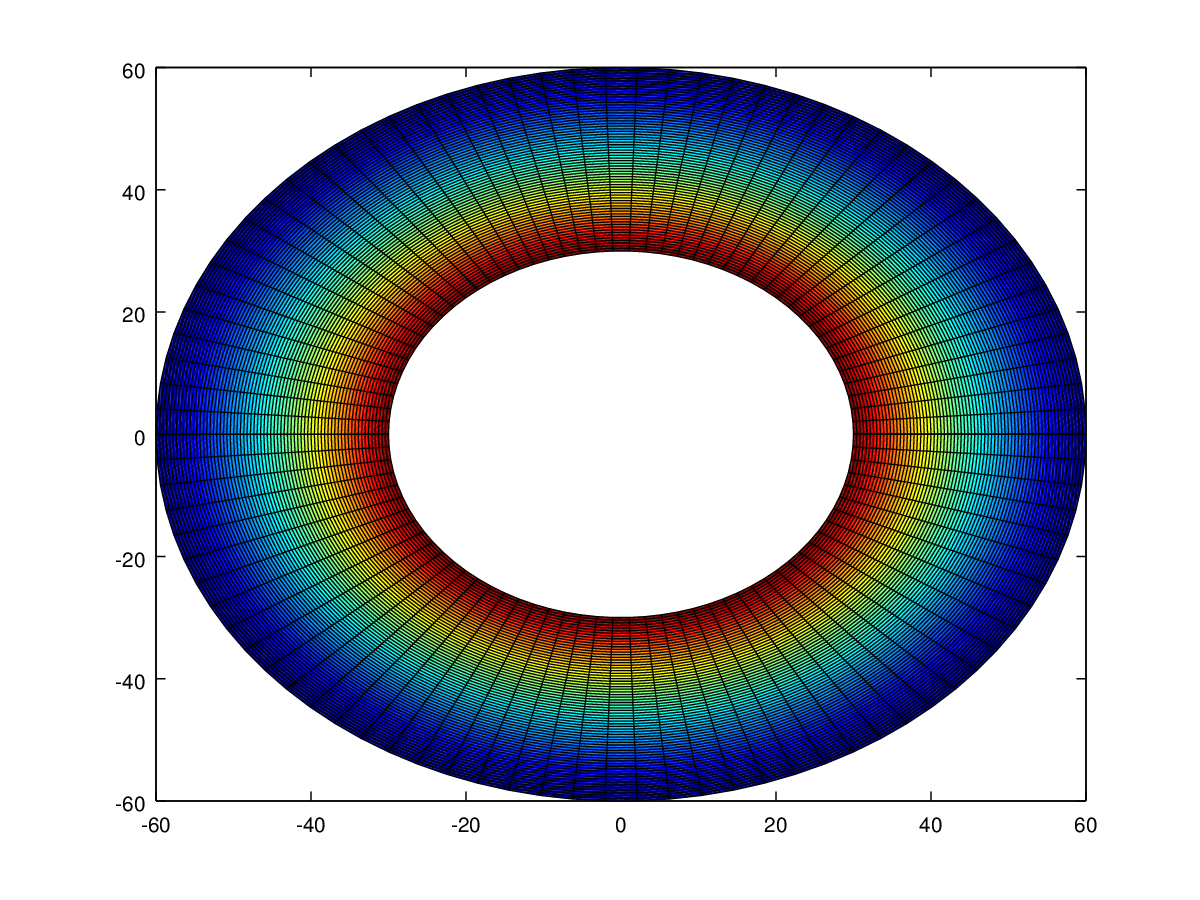
\includegraphics[height=5cm]{graficos/1/1-real.png} & 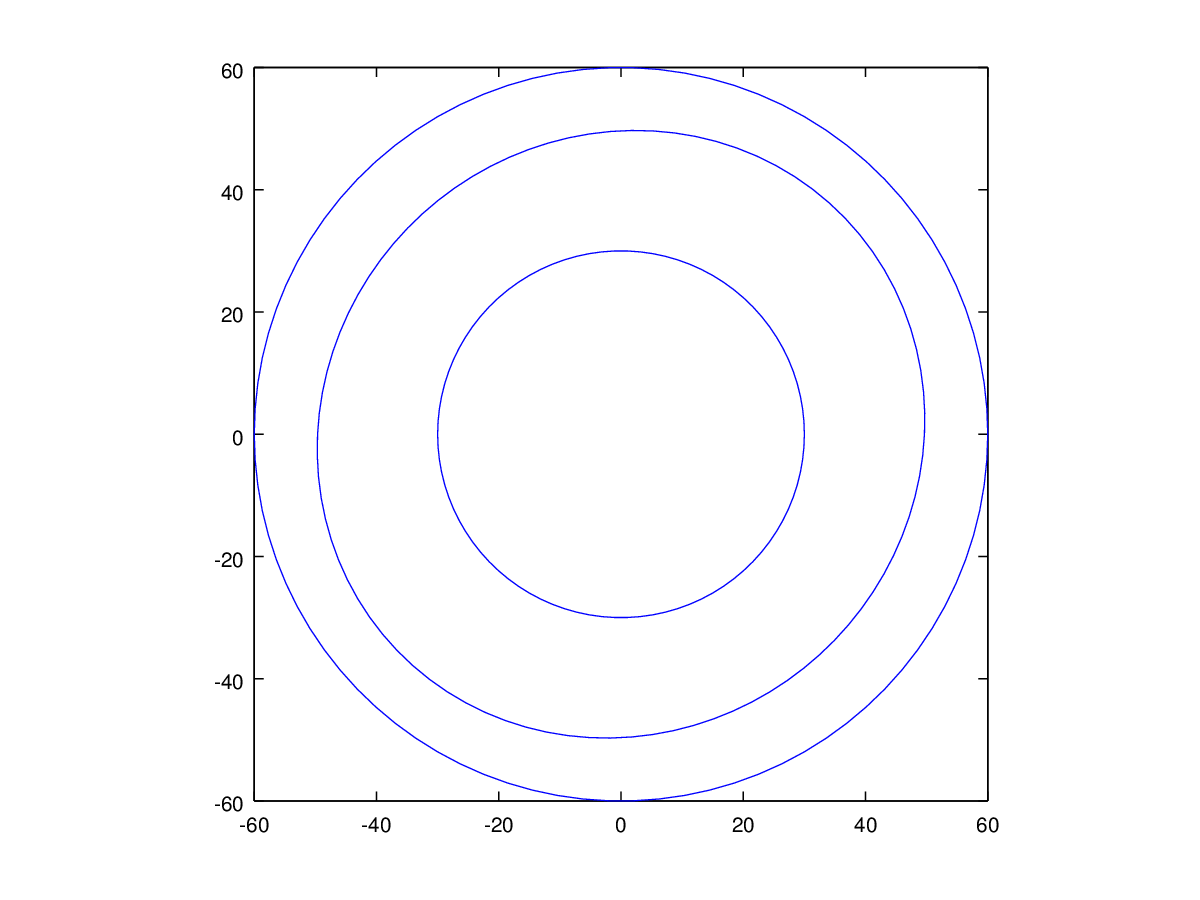
\includegraphics[height=5cm]{graficos/1/1-real-iso.png} \\
      {\small Temperaturas obtenidas} &
      {\small Posición estimada de la isoterma 500{\degree}C} \\
    \end{tabular}}

    \paragraph{Caso A} Se mantuvo constante la cantidad de radios de la discretización $m + 1 = 70$, y se tomaron instancias con diferentes cantidades de ángulos, para $n = 3, 5, 8, 10, 30, 50, 70$. Los gráficos que incluimos representan los resultados obtenidos para $n = 5, 10, 50$, reflejando las temperaturas calculadas y la ubicación estimada de la isoterma (en azul), comparada con la obtenida para el caso de contraste (en verde).

    {\centering \begin{tabular}{ccc}
      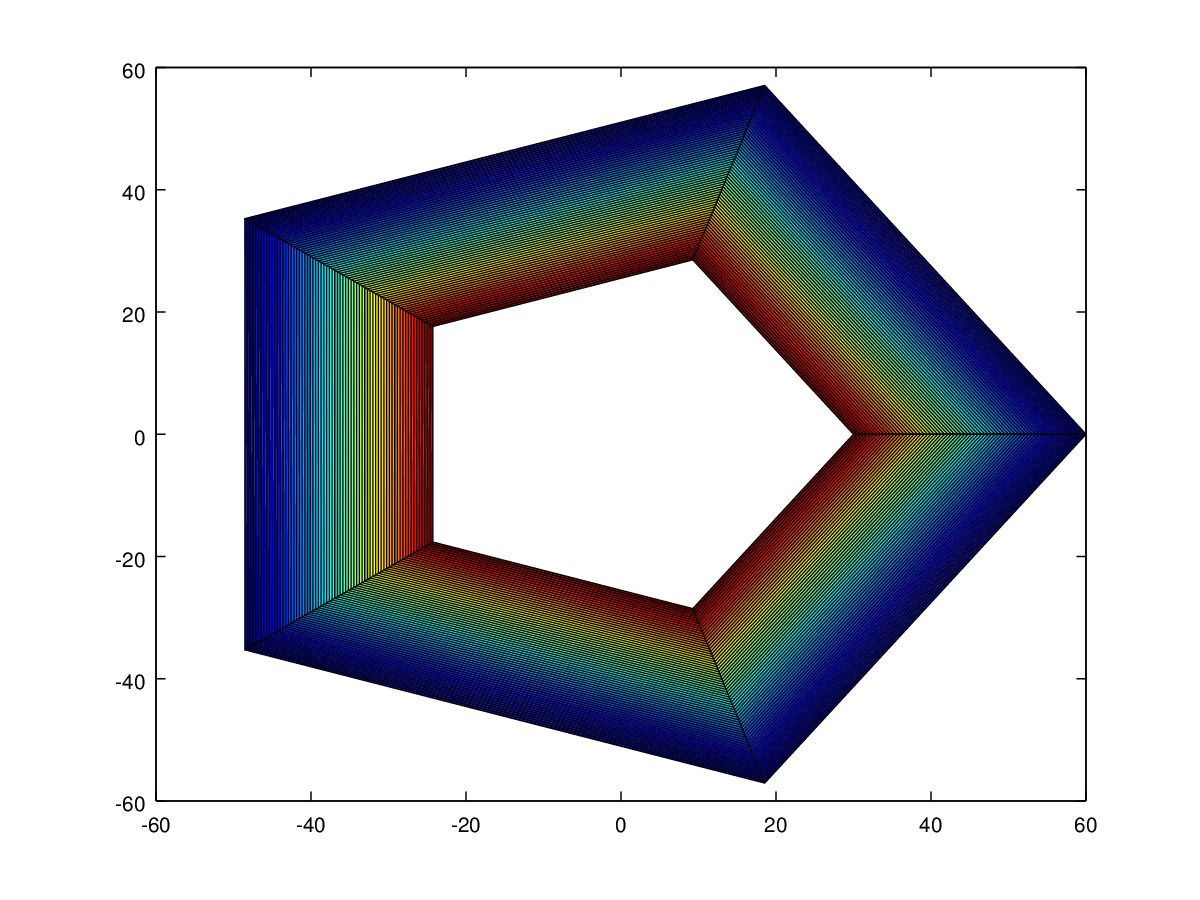
\includegraphics[width=4.5cm]{graficos/1/1a-5.png} &
      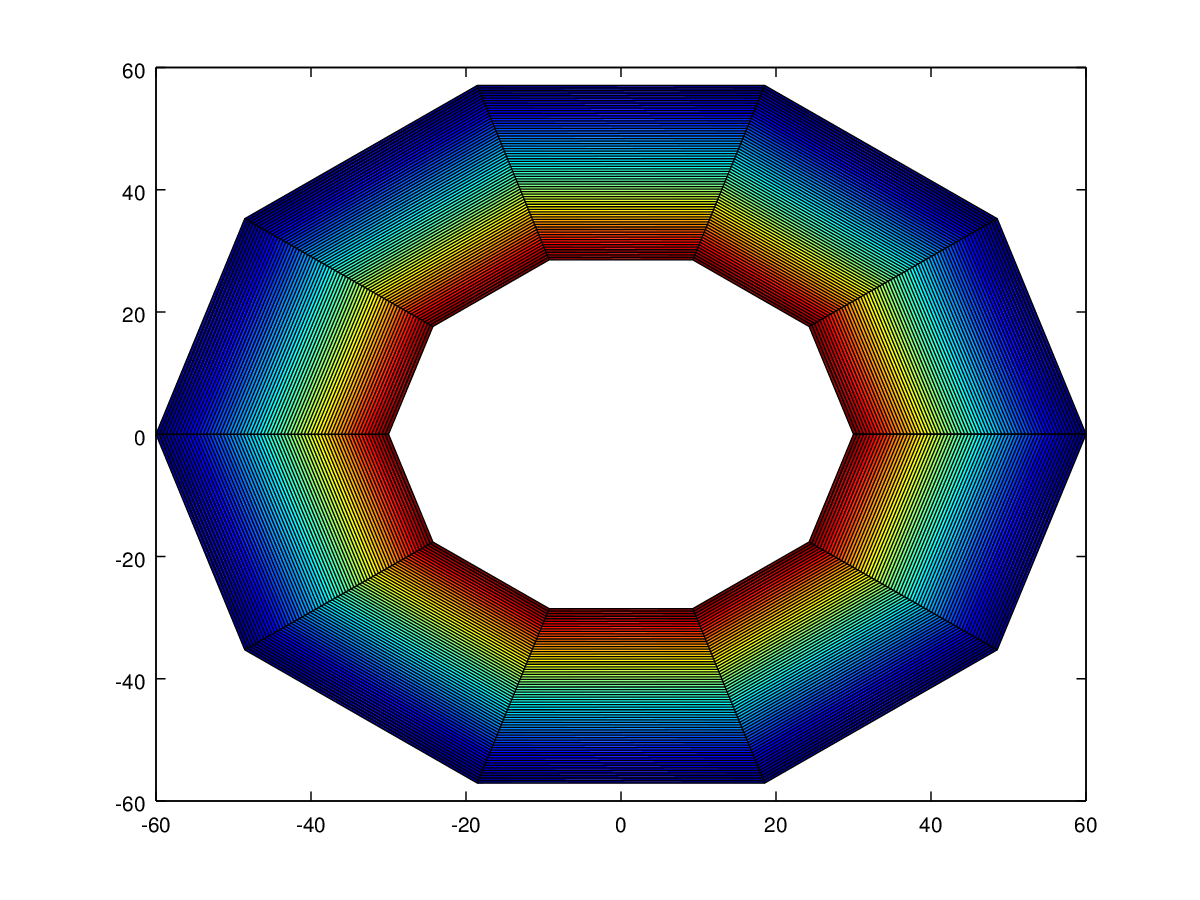
\includegraphics[width=4.5cm]{graficos/1/1a-10.png} &
      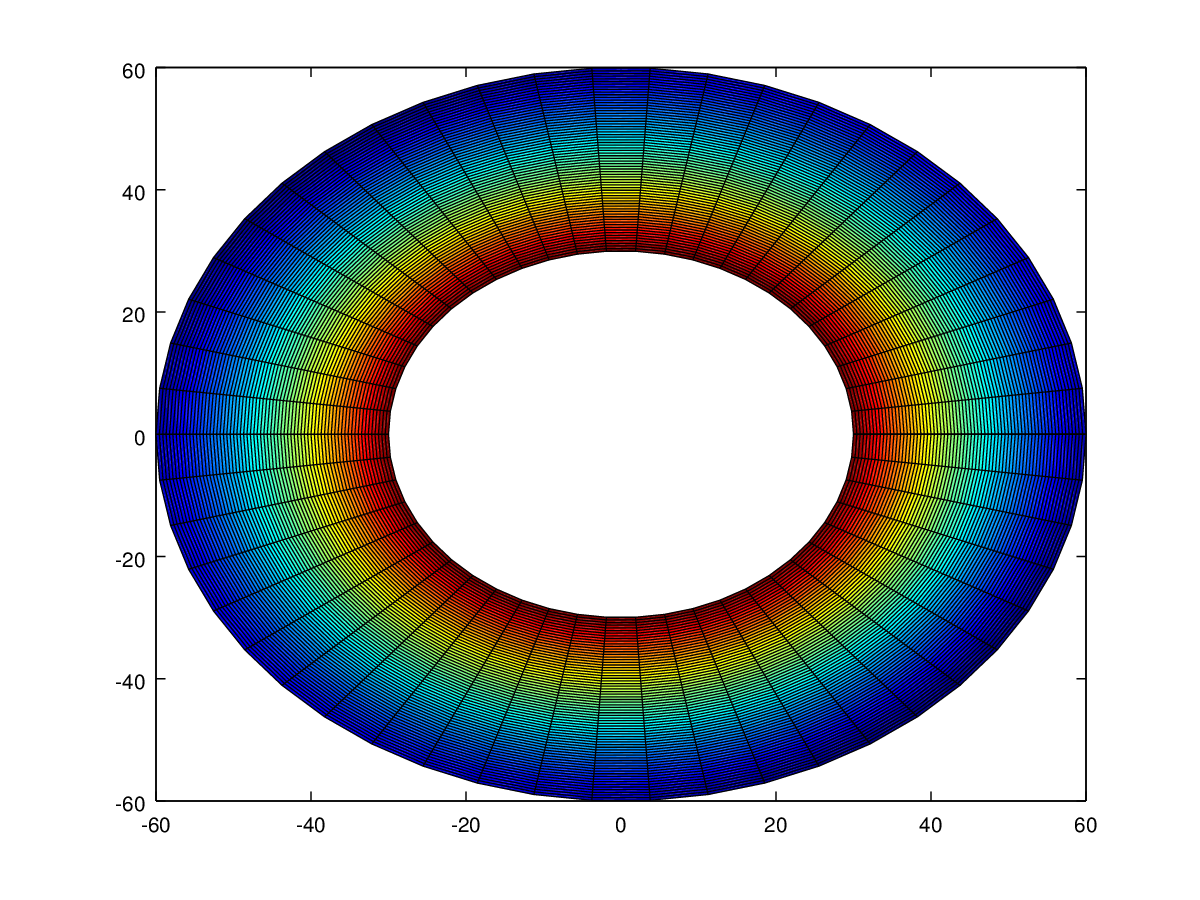
\includegraphics[width=4.5cm]{graficos/1/1a-50.png} \\
      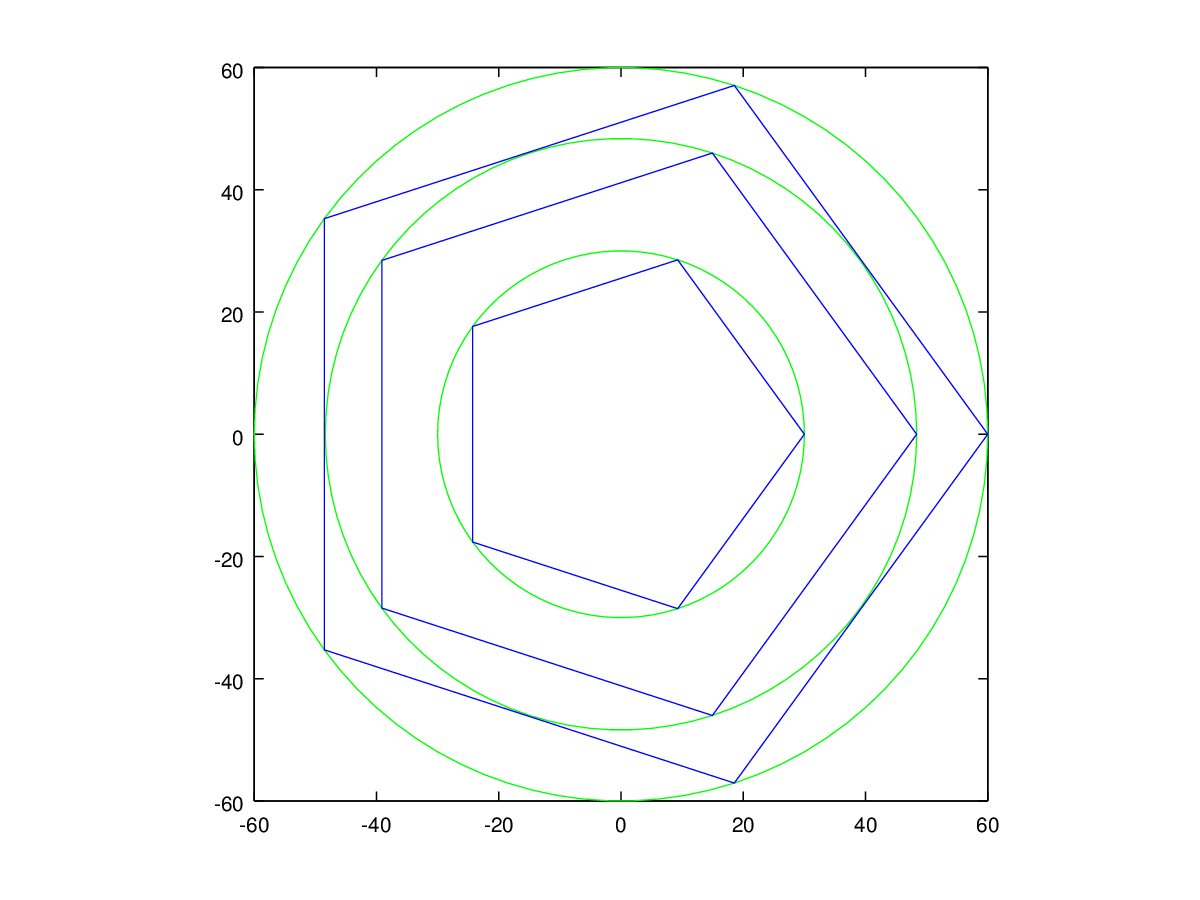
\includegraphics[width=4.5cm]{graficos/1/1a-5-iso.png} &
      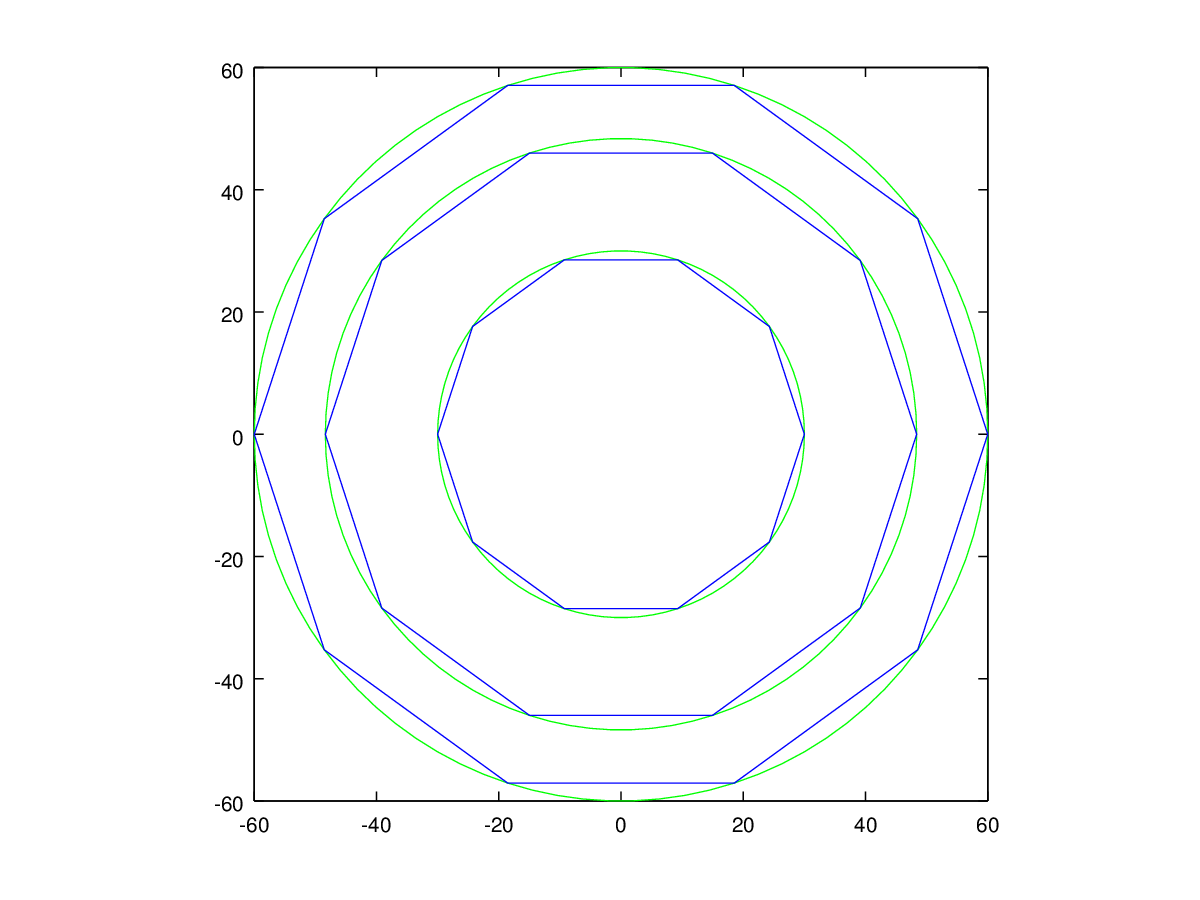
\includegraphics[width=4.5cm]{graficos/1/1a-10-iso.png} &
      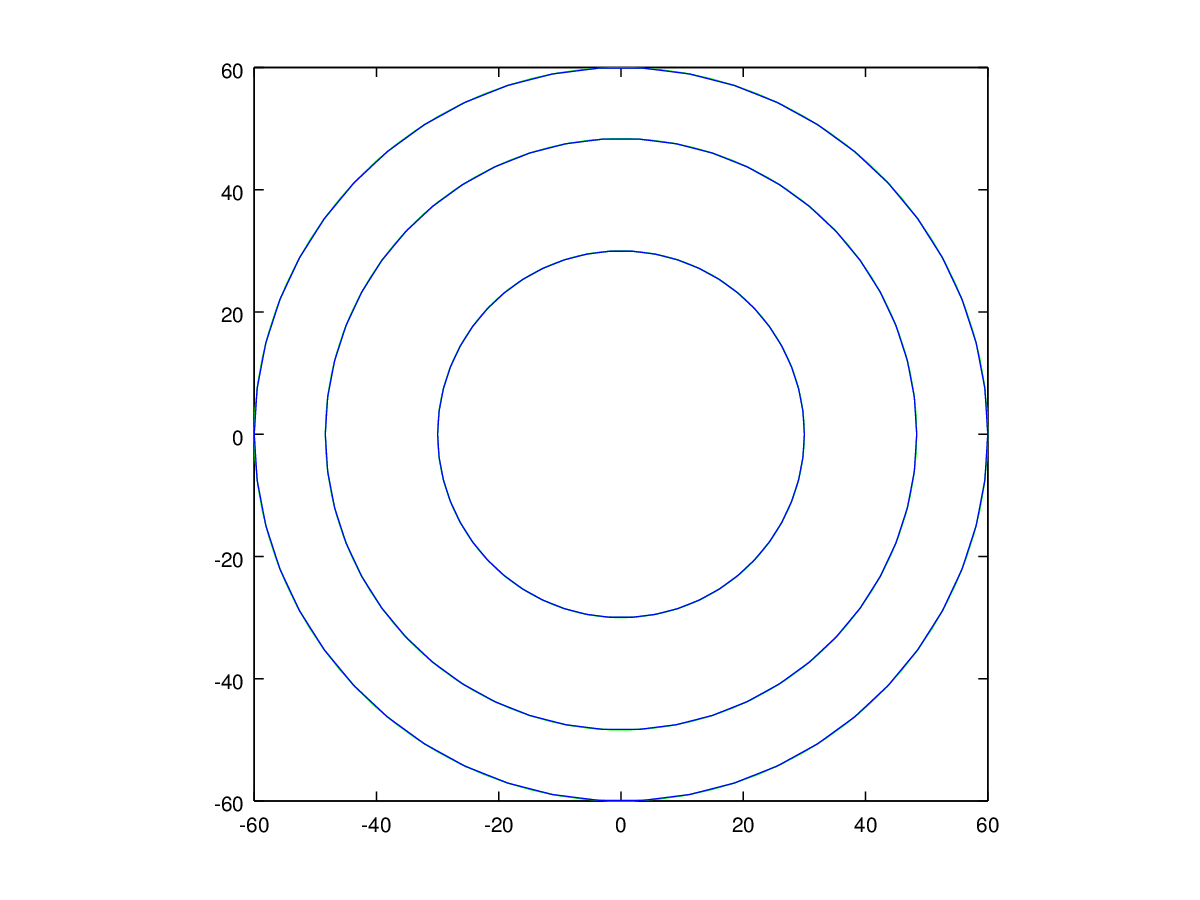
\includegraphics[width=4.5cm]{graficos/1/1a-50-iso.png} \\
      {\small $n = 5$} &
      {\small $n = 10$} &
      {\small $n = 50$} \\
    \end{tabular}}

    \paragraph{Caso B} Se mantuvo constante la cantidad de ángulos de la discretización $n = 90$, y se tomaron instancias con diferentes cantidades de ángulos, para $m + 1 = 3, 5, 8, 10, 30, 50$. Los gráficos que incluimos representan los resultados obtenidos para $m + 1 = 3, 8, 30$, reflejando las temperaturas calculadas y la ubicación estimada de la isoterma (en azul), comparada con la obtenida para el caso de contraste (en verde).

    {\centering \begin{tabular}{ccc}
      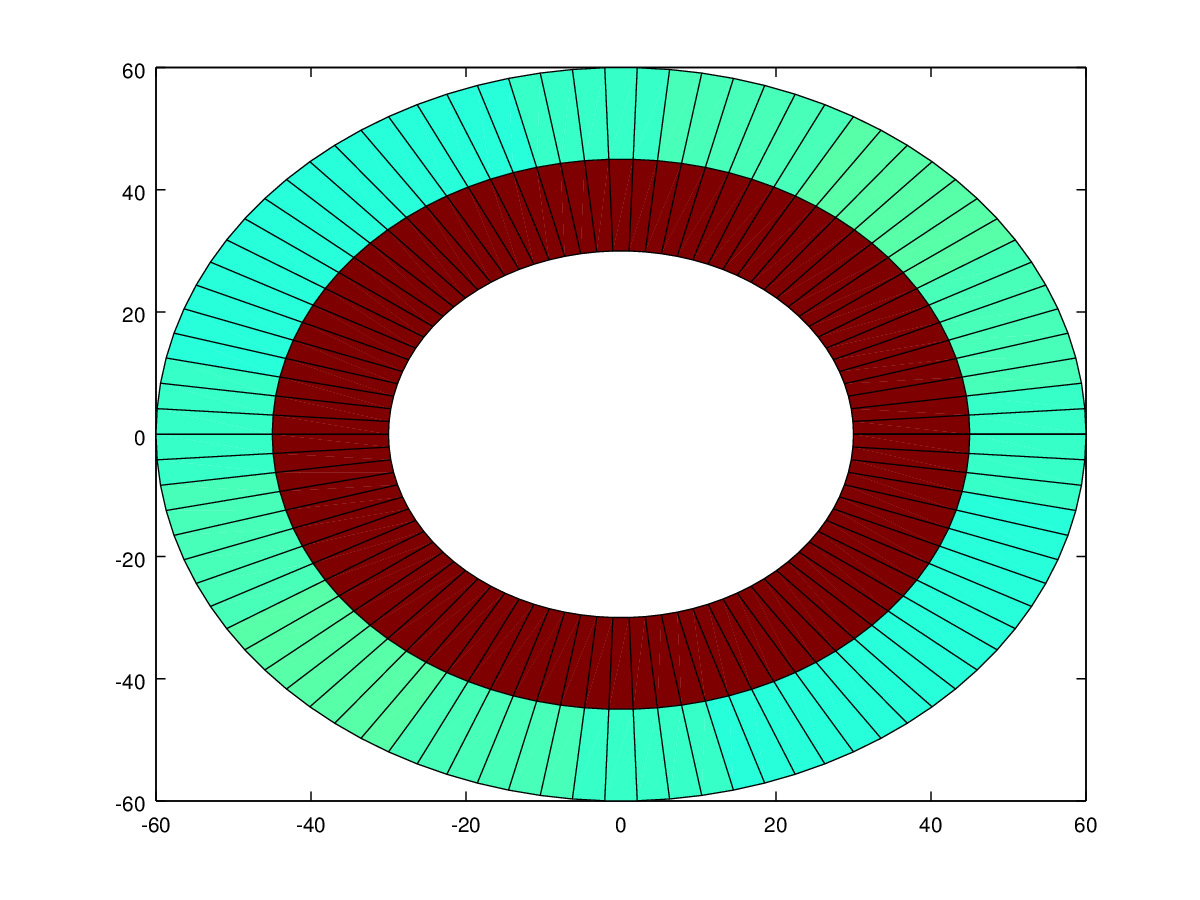
\includegraphics[width=4.5cm]{graficos/1/1b-3.png} &
      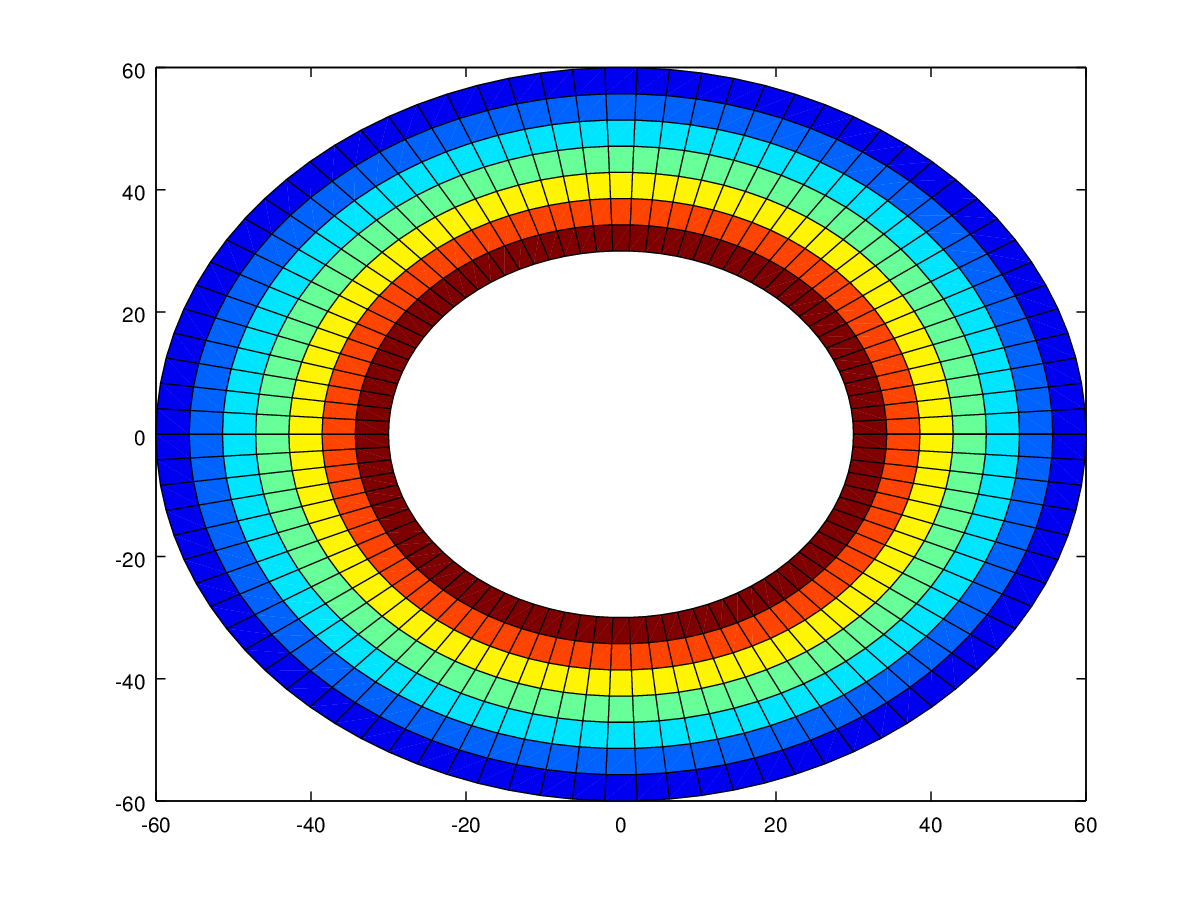
\includegraphics[width=4.5cm]{graficos/1/1b-8.png} &
      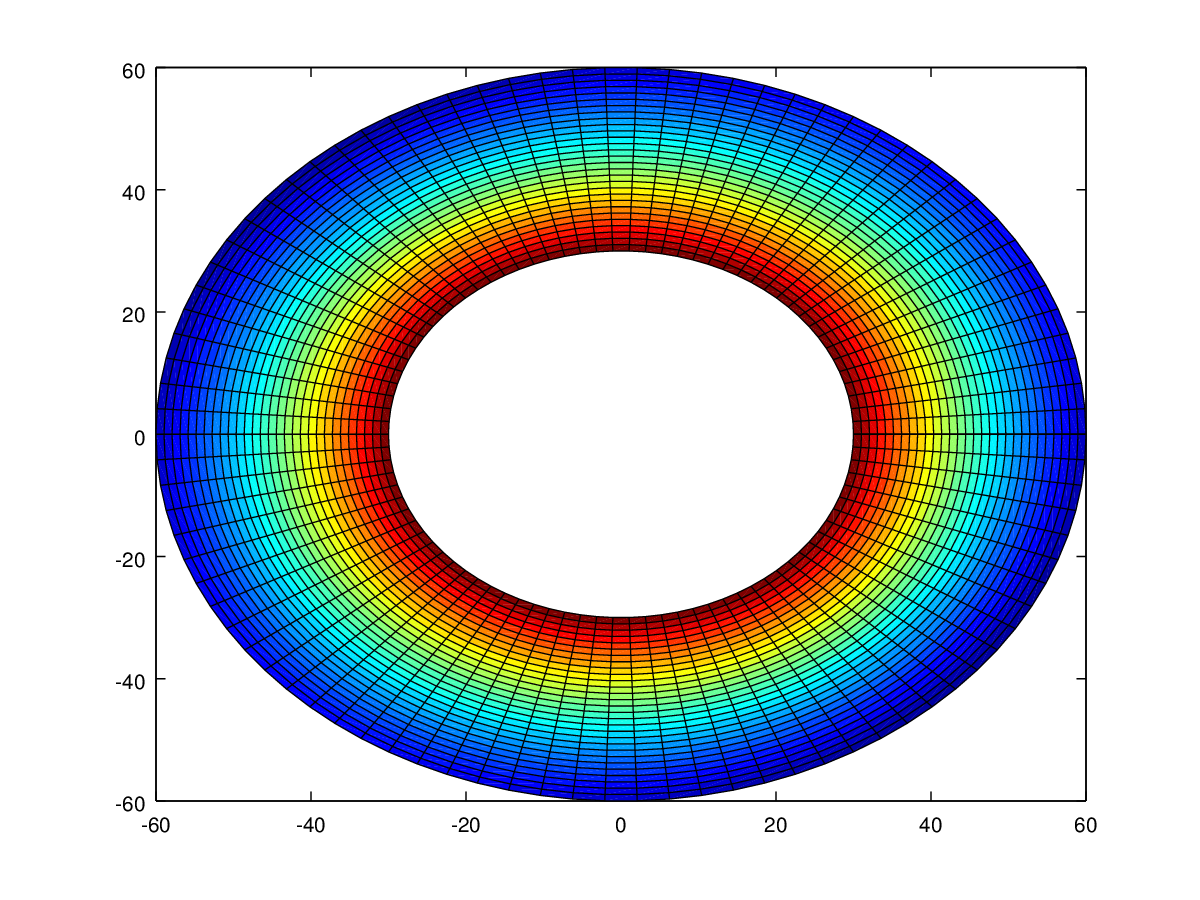
\includegraphics[width=4.5cm]{graficos/1/1b-30.png} \\
      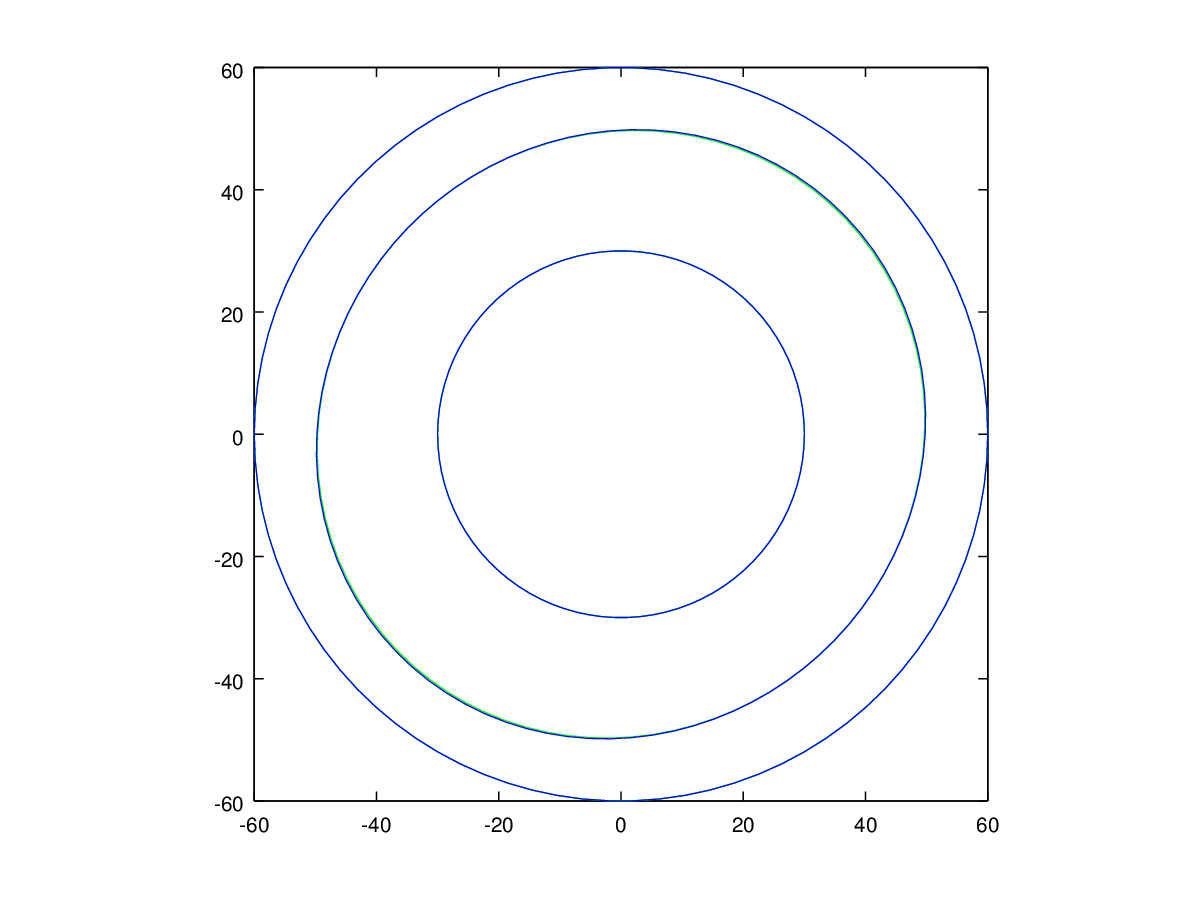
\includegraphics[width=4.5cm]{graficos/1/1b-3-iso.png} &
      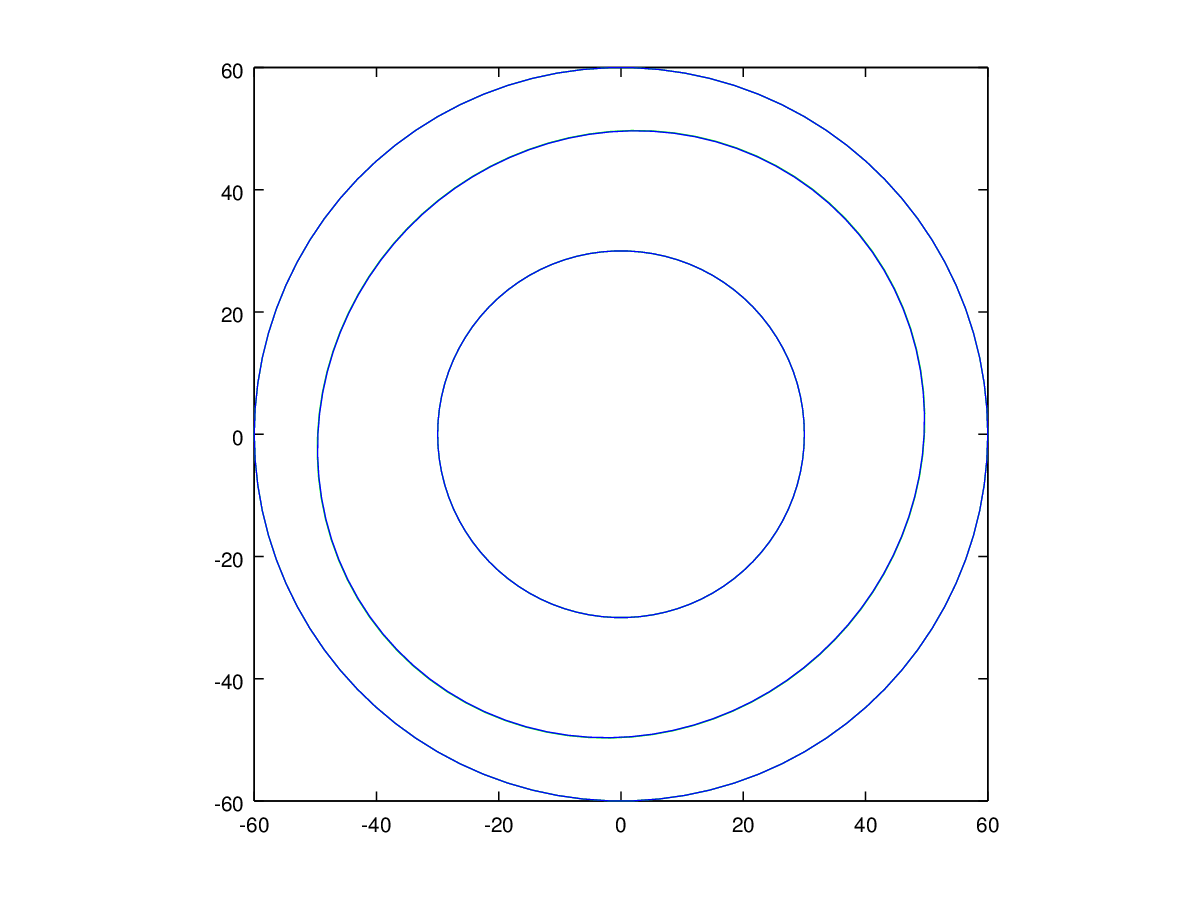
\includegraphics[width=4.5cm]{graficos/1/1b-8-iso.png} &
      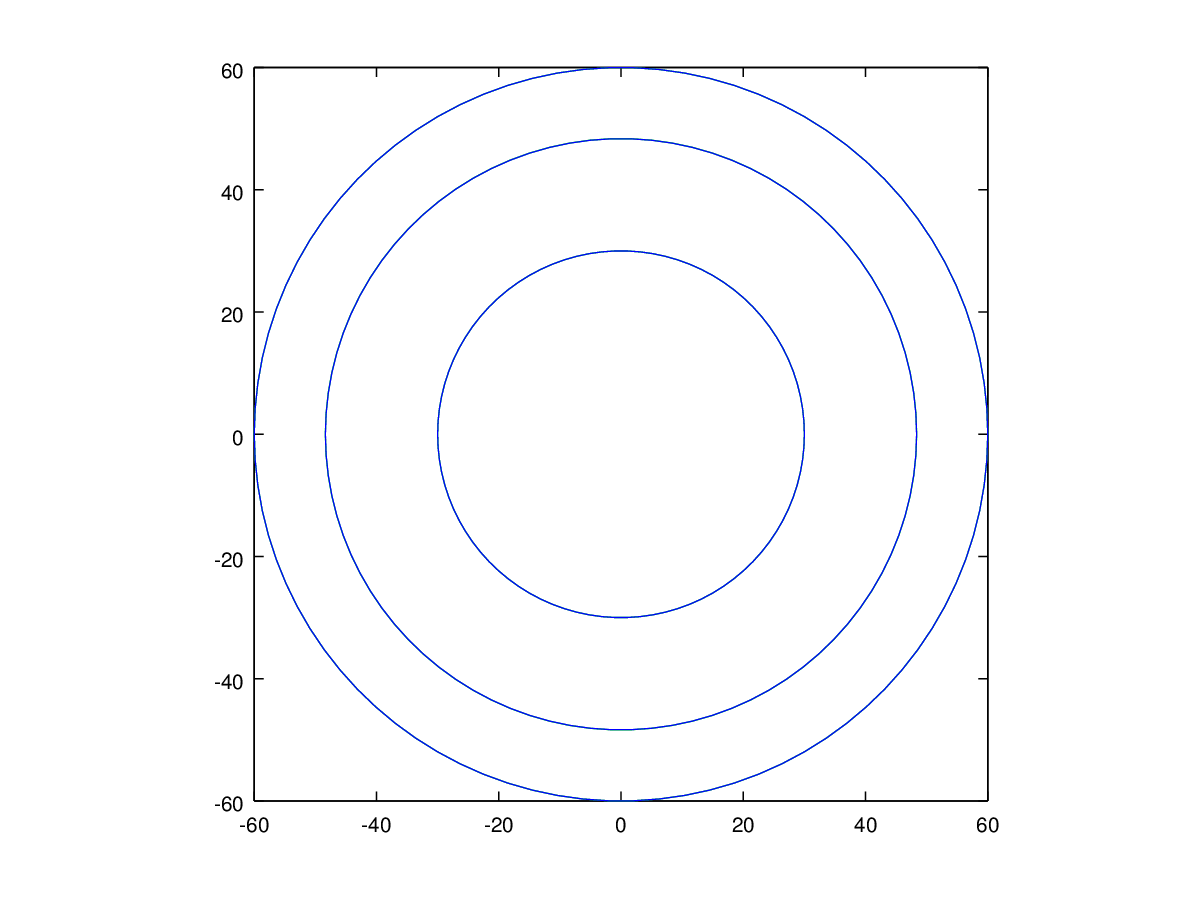
\includegraphics[width=4.5cm]{graficos/1/1b-30-iso.png} \\
      {\small $n = 3$} &
      {\small $n = 8$} &
      {\small $n = 30$} \\
    \end{tabular}}

  \subsubsection*{Experimento 2: Posición de la isoterma según granularidad}

    Para ambos casos se consideraron instancias de prueba con los siguientes parámetros: $r_i = 30$, $r_e = 60$, $T_i = 1500$, $iso = 500$. Se generó una instancia de prueba con una temperatura externa variable entre 50 y 200{\degree}C
    % , con $T_e(\theta) = 125 + 75 \sin(2\theta)$ 
    en todos los puntos $(r_e, \theta)$ de la discretización.
    En primer lugar, se calculó la solución del sistema y la posición estimada de la isoterma para una discretización considerablemente granular, con $m + 1 = 70$ y $n = 90$, para utilizar como caso de contraste. Reproducimos los gráficos que representan las temperaturas calculadas para todos los puntos de la discretización y la ubicación estimada de la isoterma.

    {\centering \begin{tabular}{cc}
      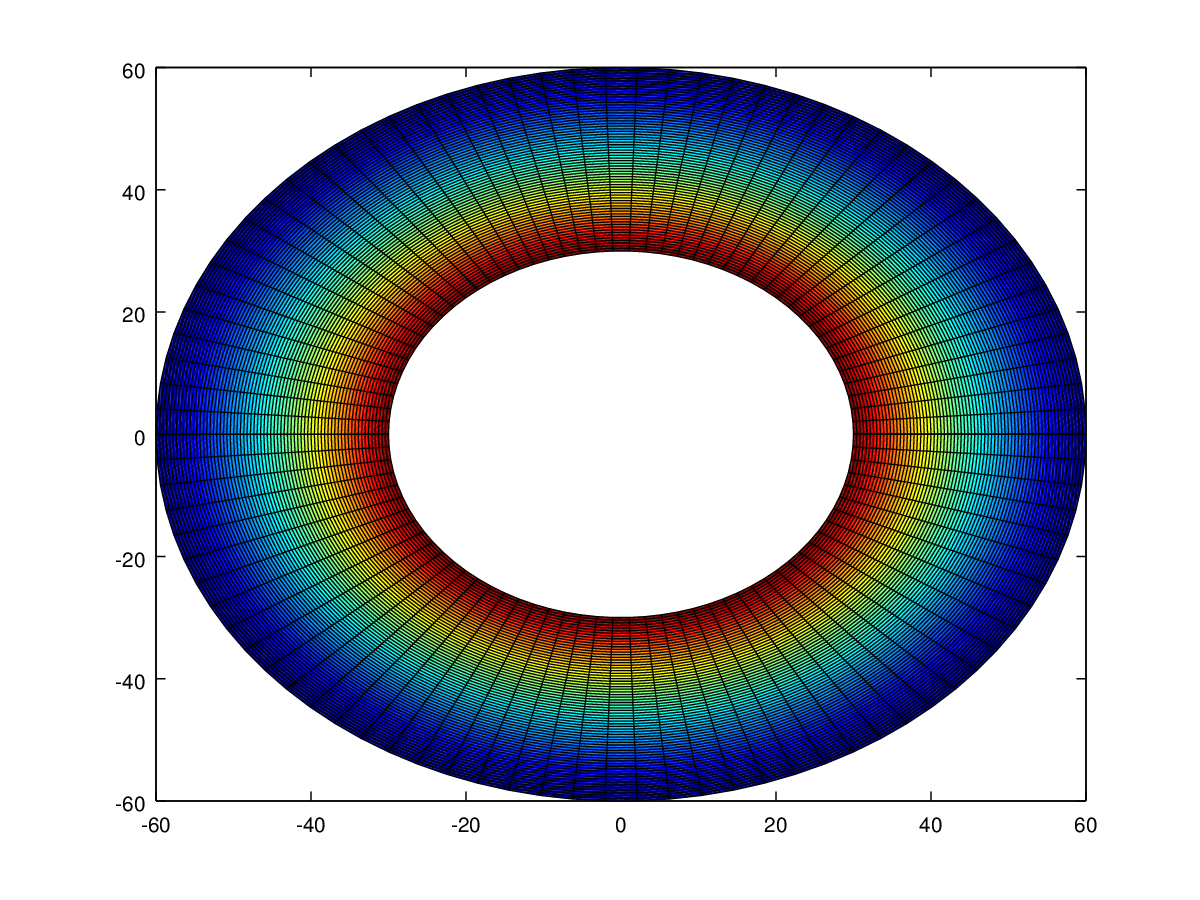
\includegraphics[height=5cm]{graficos/2/2-real.png} & 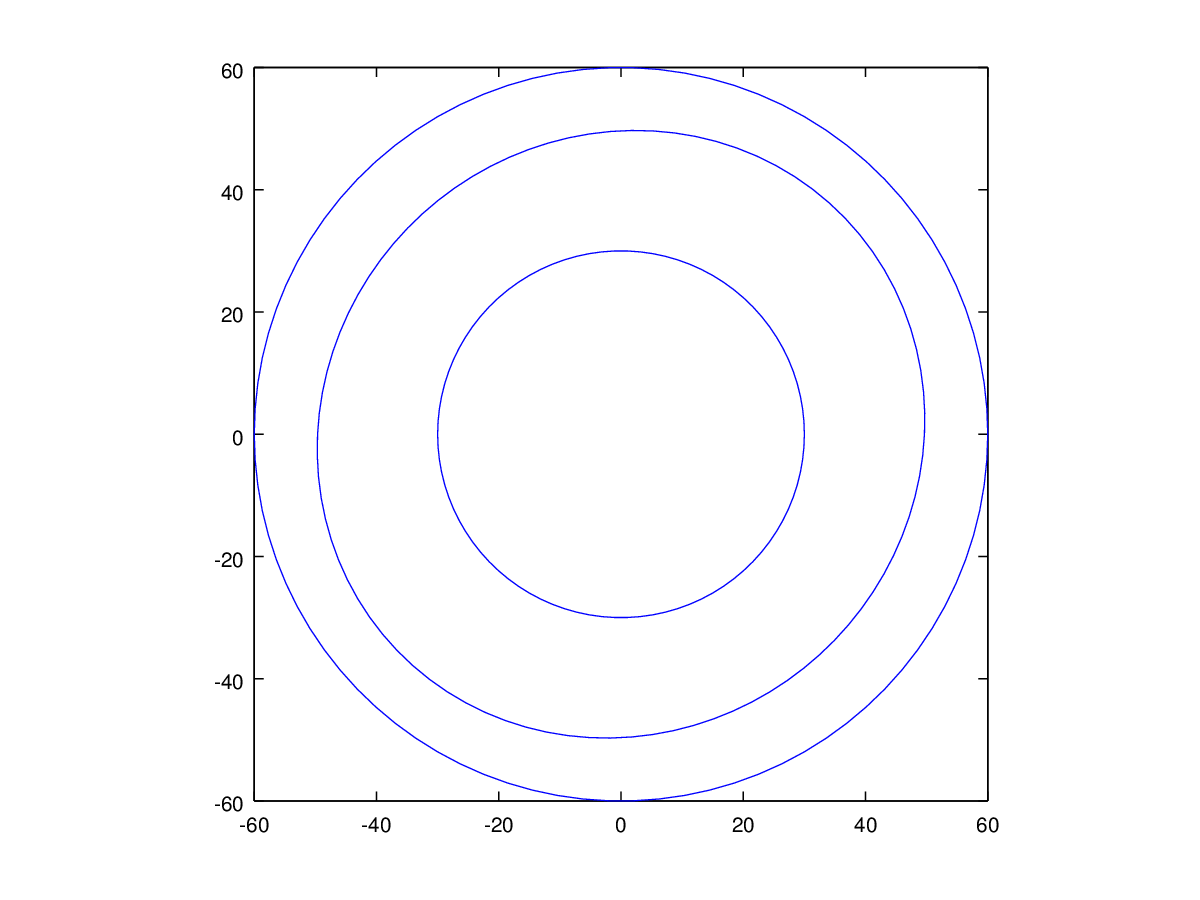
\includegraphics[height=5cm]{graficos/2/2-real-iso.png} \\
      {\small Temperaturas obtenidas} &
      {\small Posición estimada de la isoterma 500{\degree}C} \\
    \end{tabular}}

    \paragraph{Caso A} Se mantuvo constante la cantidad de radios de la discretización $m + 1 = 70$, y se tomaron instancias con diferentes cantidades de ángulos, para $n = 3, 5, 8, 10, 30, 50, 70$. Los gráficos que incluimos representan los resultados obtenidos para $n = 5, 10, 50$, reflejando las temperaturas calculadas y la ubicación estimada de la isoterma (en azul), comparada con la obtenida para el caso de contraste (en verde).

    {\centering \begin{tabular}{ccc}
      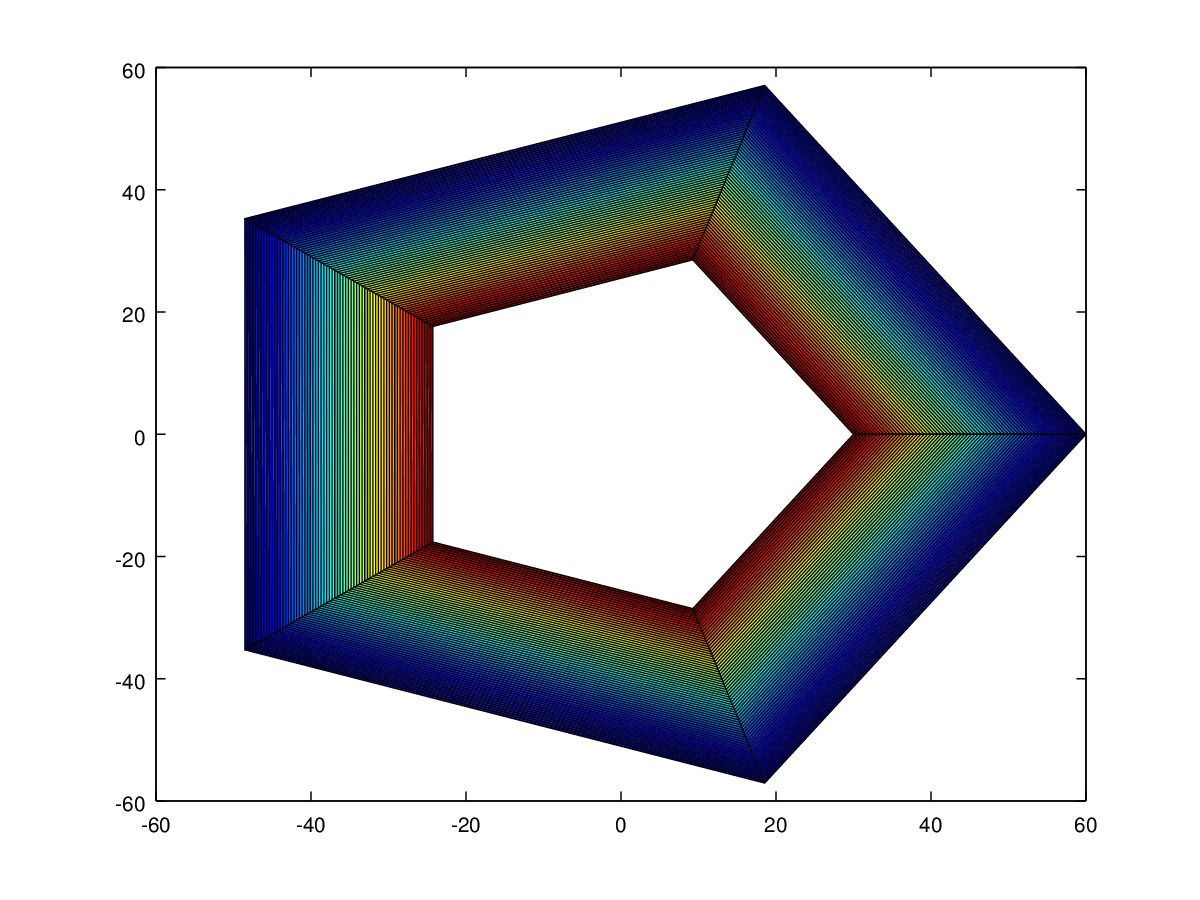
\includegraphics[width=4.5cm]{graficos/2/2a-5.png} &
      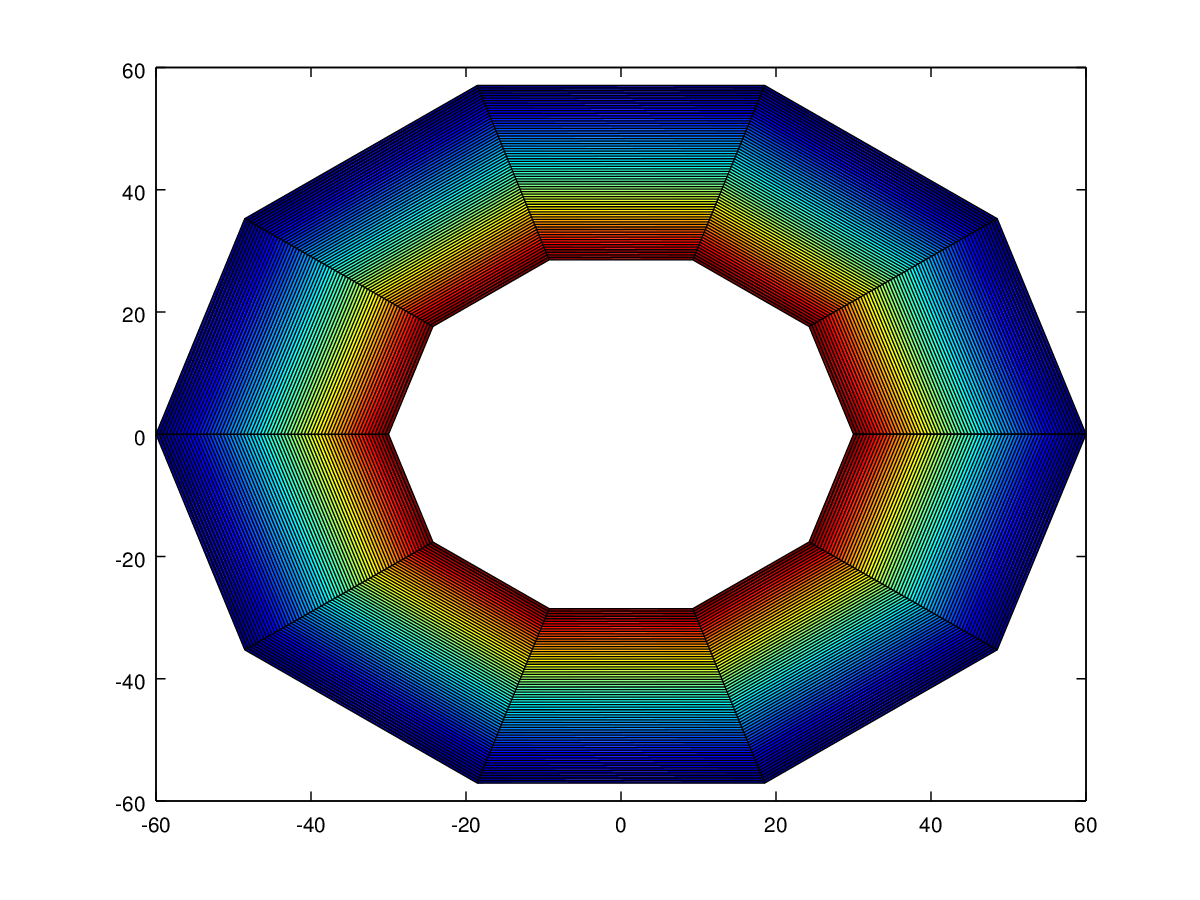
\includegraphics[width=4.5cm]{graficos/2/2a-10.png} &
      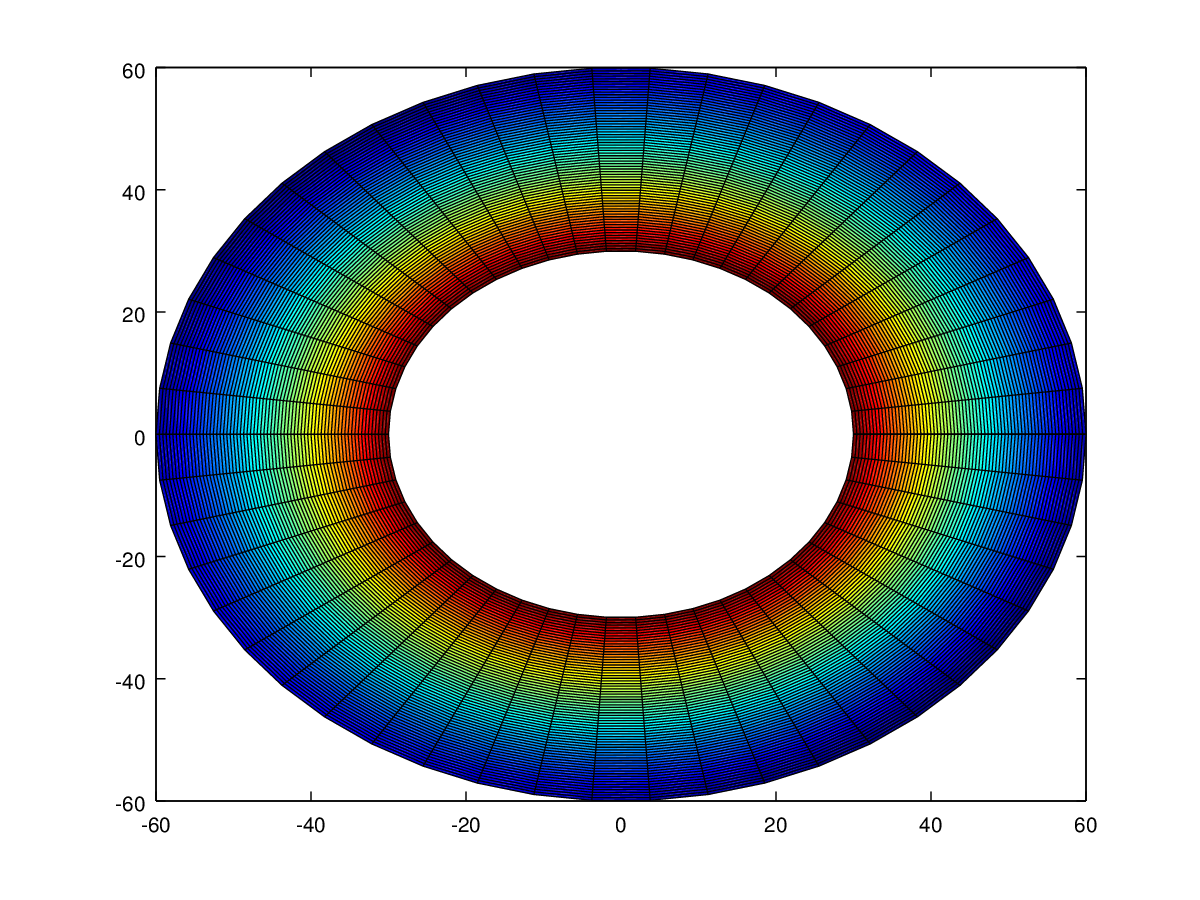
\includegraphics[width=4.5cm]{graficos/2/2a-50.png} \\
      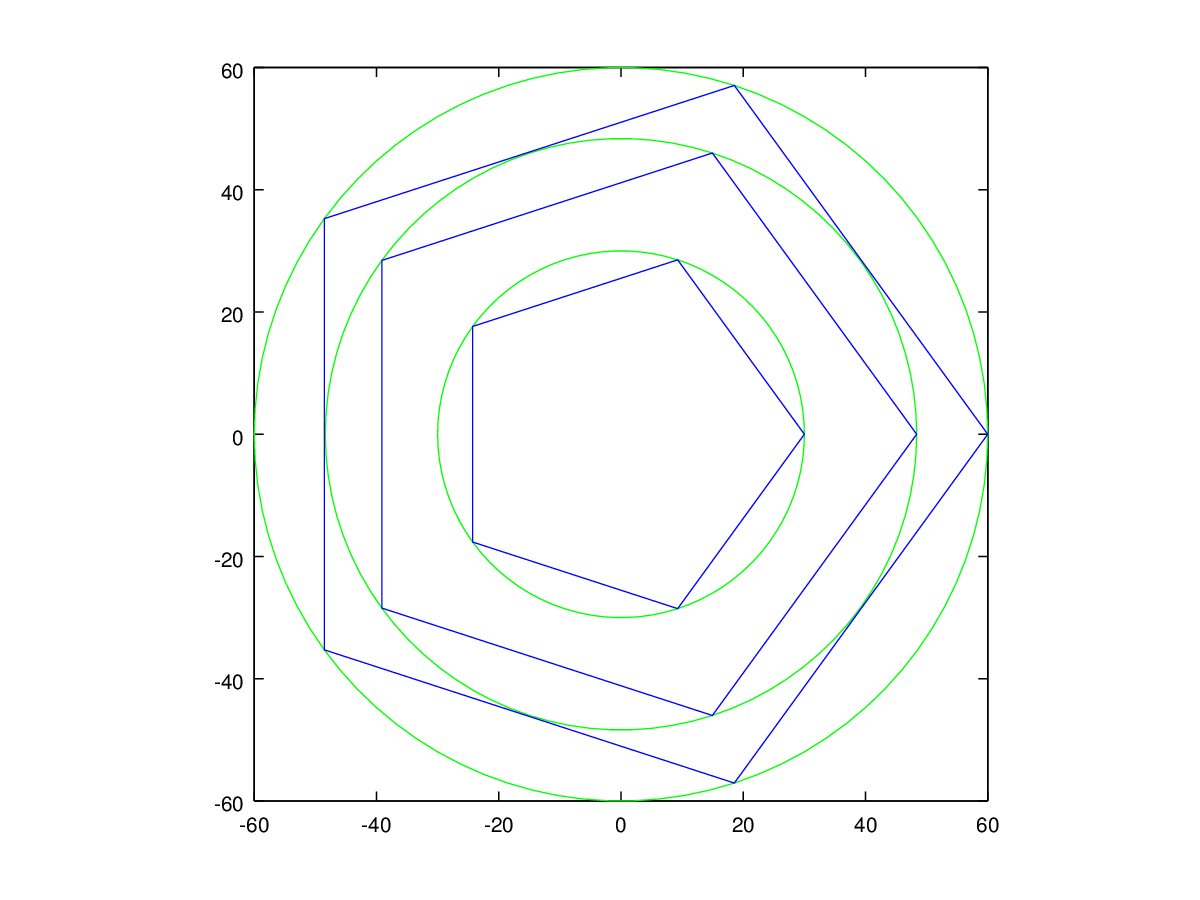
\includegraphics[width=4.5cm]{graficos/2/2a-5-iso.png} &
      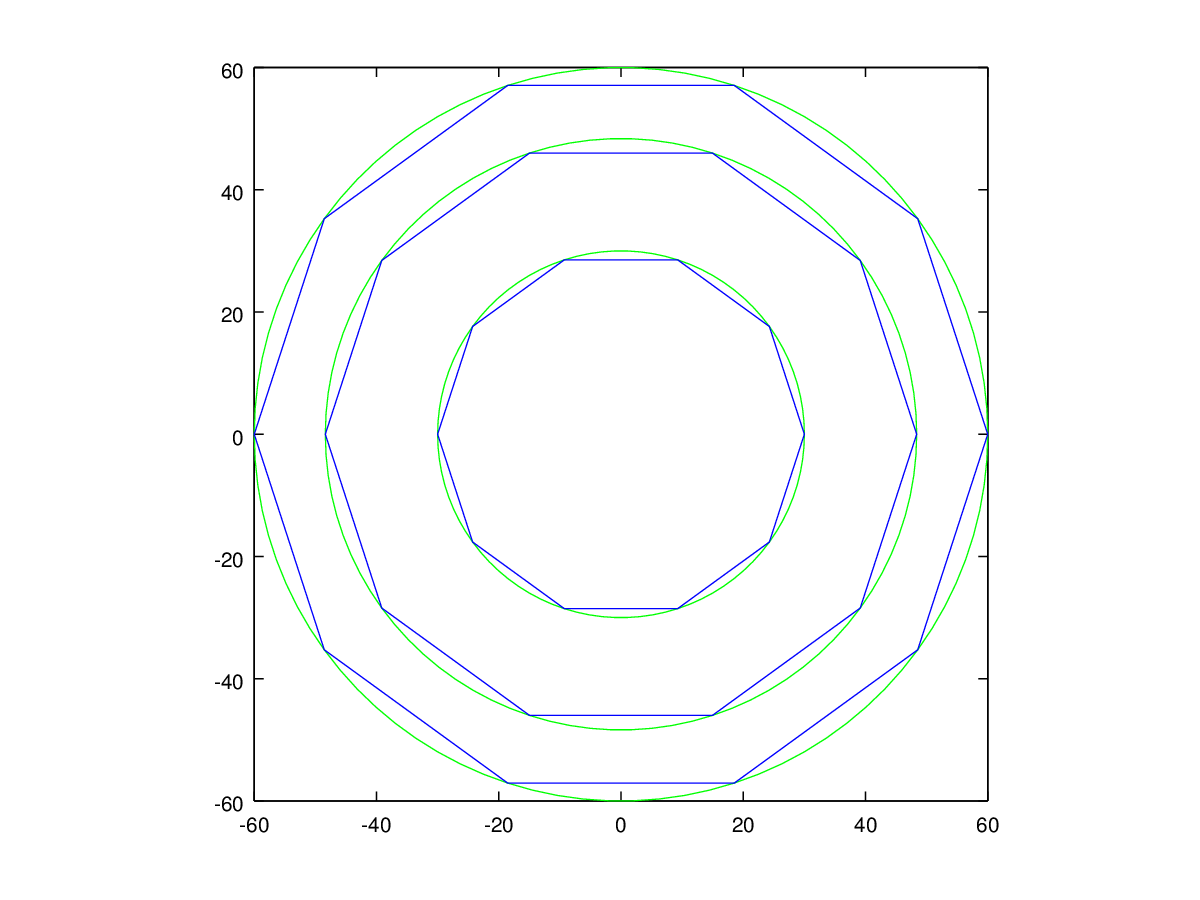
\includegraphics[width=4.5cm]{graficos/2/2a-10-iso.png} &
      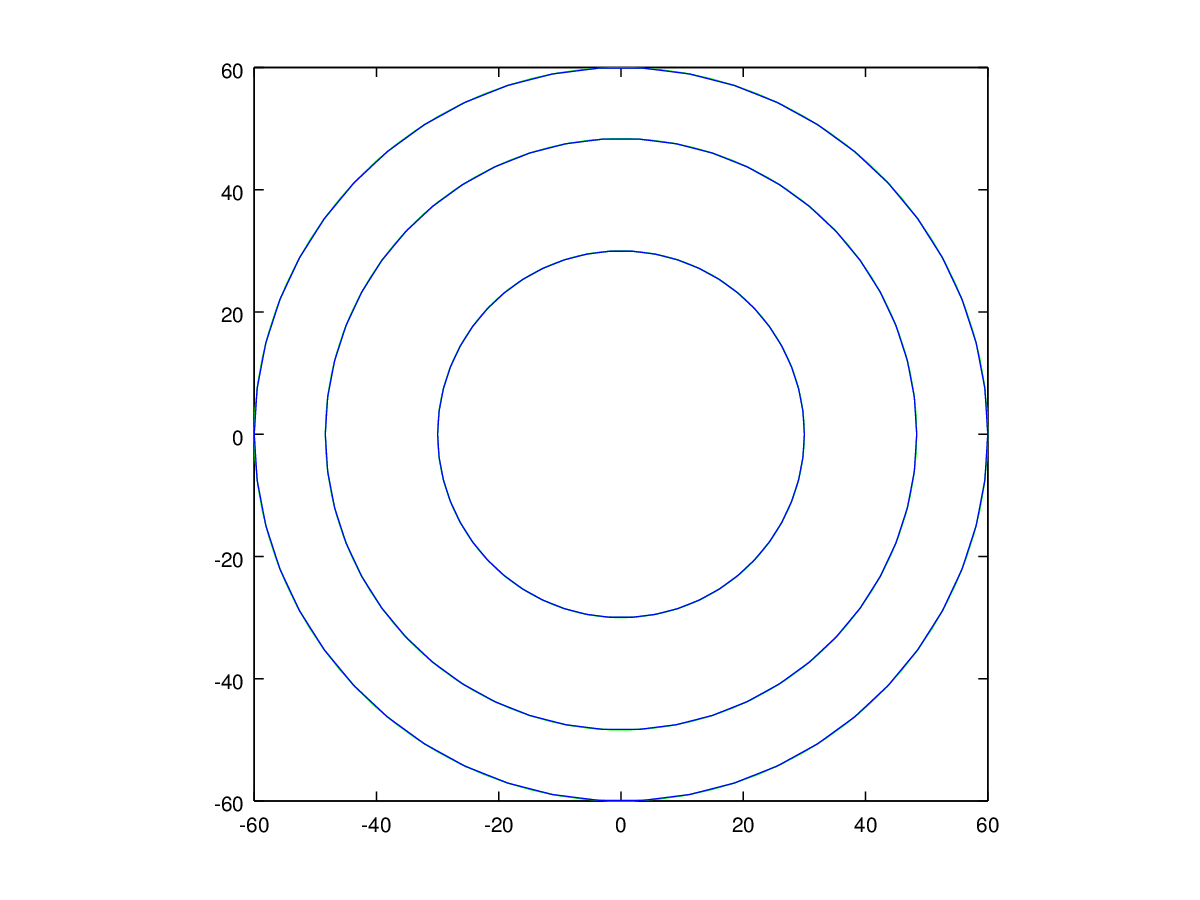
\includegraphics[width=4.5cm]{graficos/2/2a-50-iso.png} \\
      {\small $n = 5$} &
      {\small $n = 10$} &
      {\small $n = 50$} \\
    \end{tabular}}

    \paragraph{Caso B} Se mantuvo constante la cantidad de ángulos de la discretización $n = 90$, y se tomaron instancias con diferentes cantidades de ángulos, para $m + 1 = 3, 5, 8, 10, 30, 50$. Los gráficos que incluimos representan los resultados obtenidos para $m + 1 = 3, 8, 30$, reflejando las temperaturas calculadas y la ubicación estimada de la isoterma (en azul), comparada con la obtenida para el caso de contraste (en verde).

    {\centering \begin{tabular}{ccc}
      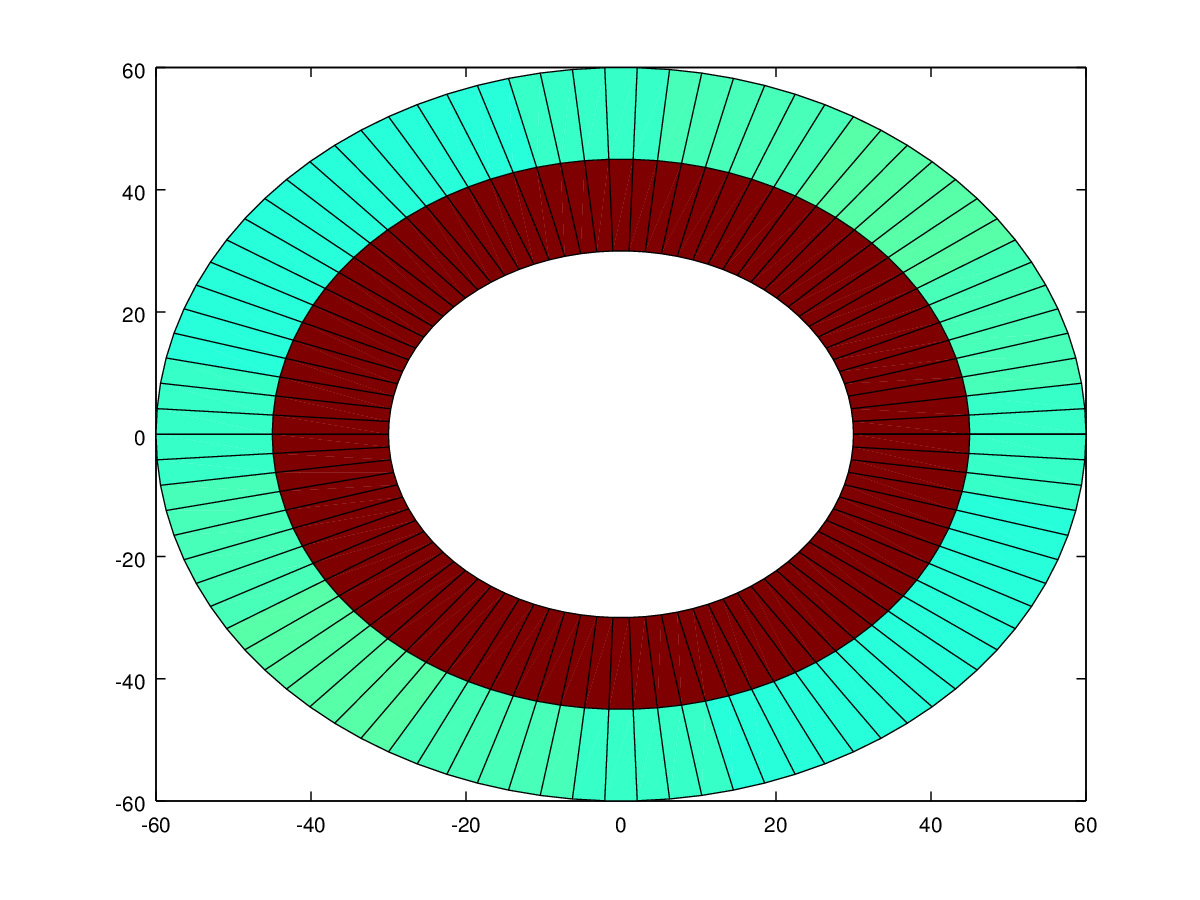
\includegraphics[width=4.5cm]{graficos/1/1b-3.png} &
      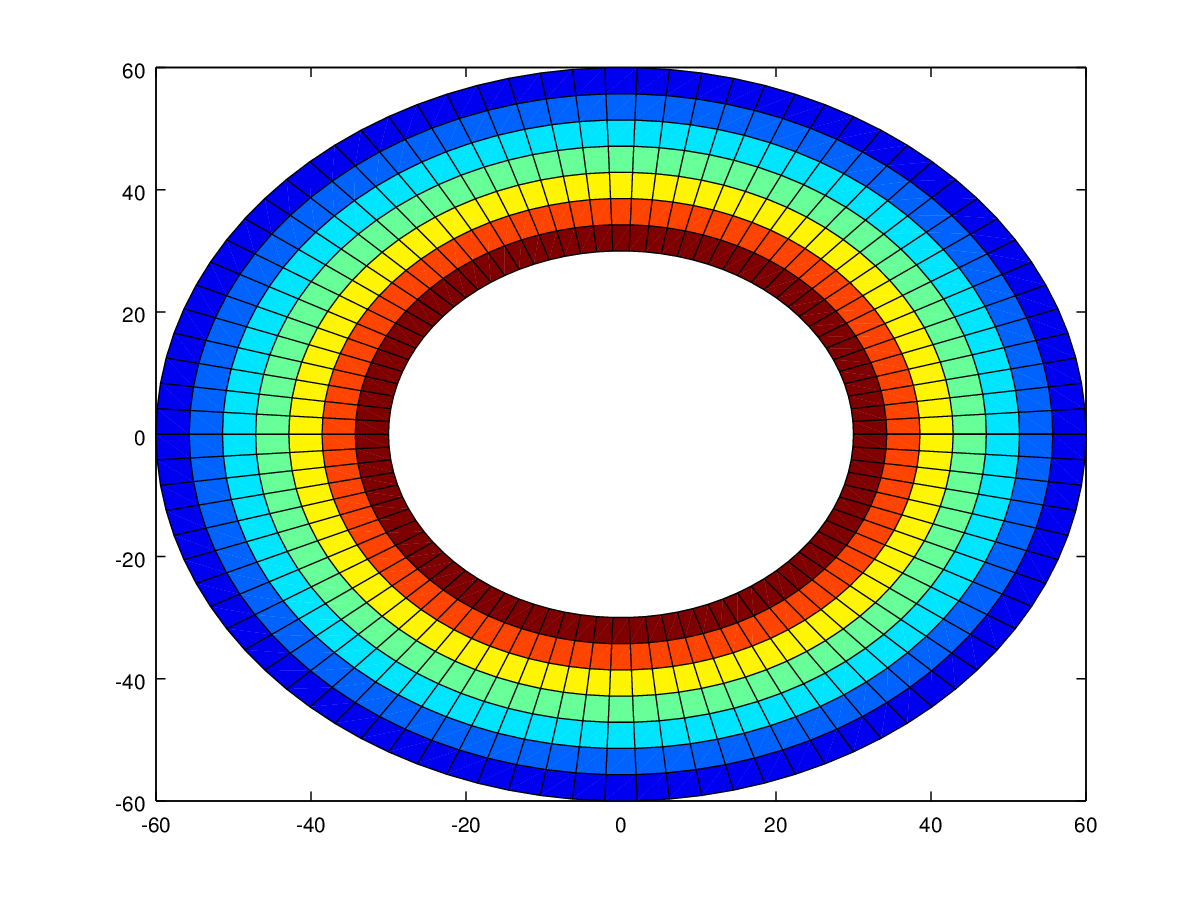
\includegraphics[width=4.5cm]{graficos/1/1b-8.png} &
      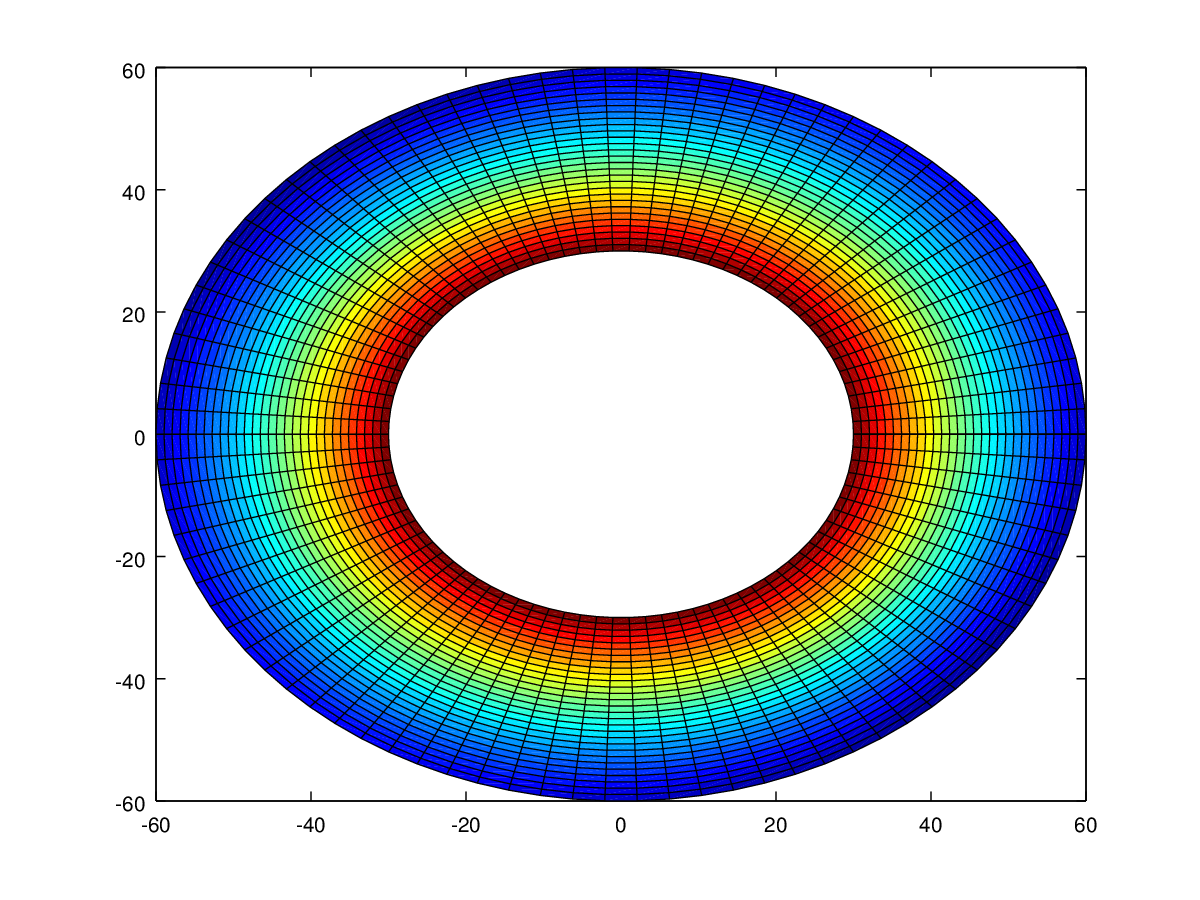
\includegraphics[width=4.5cm]{graficos/1/1b-30.png} \\
      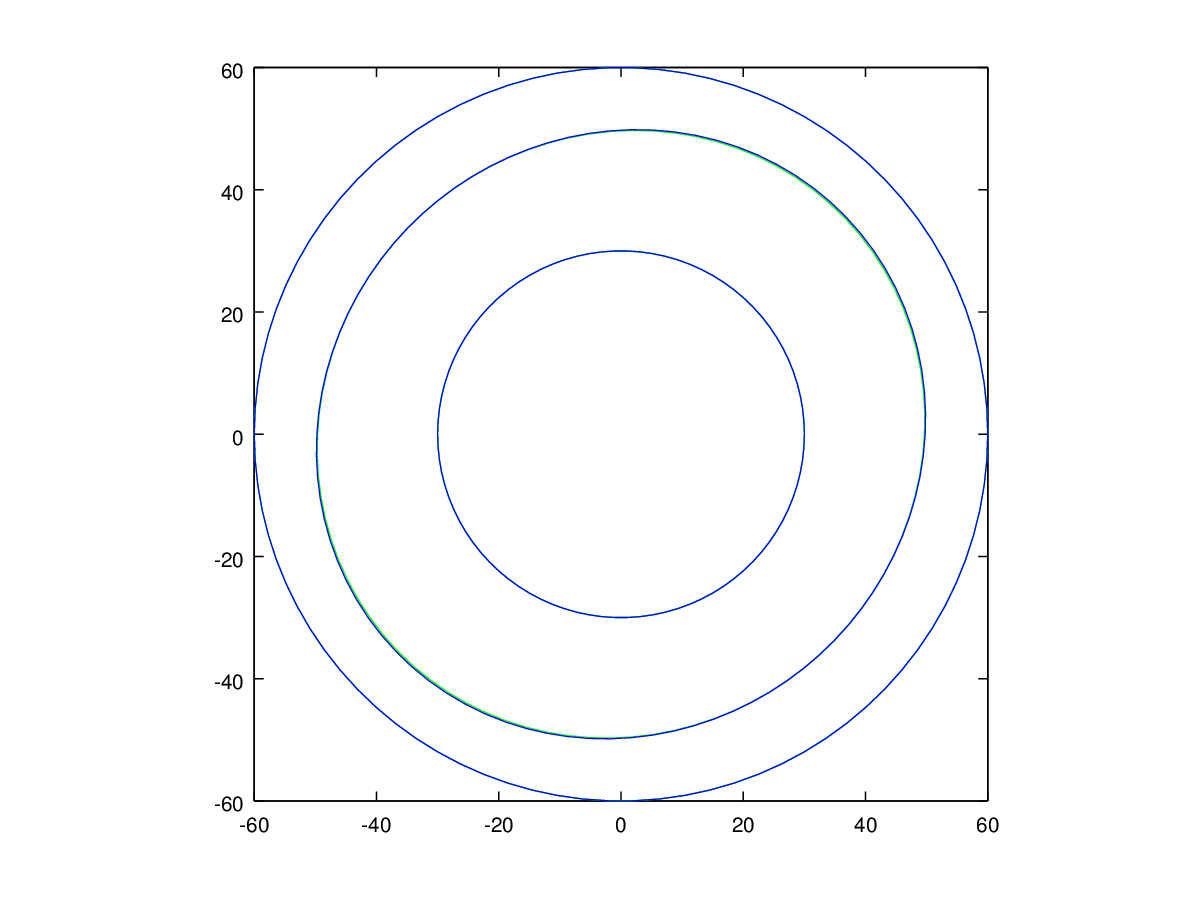
\includegraphics[width=4.5cm]{graficos/1/1b-3-iso.png} &
      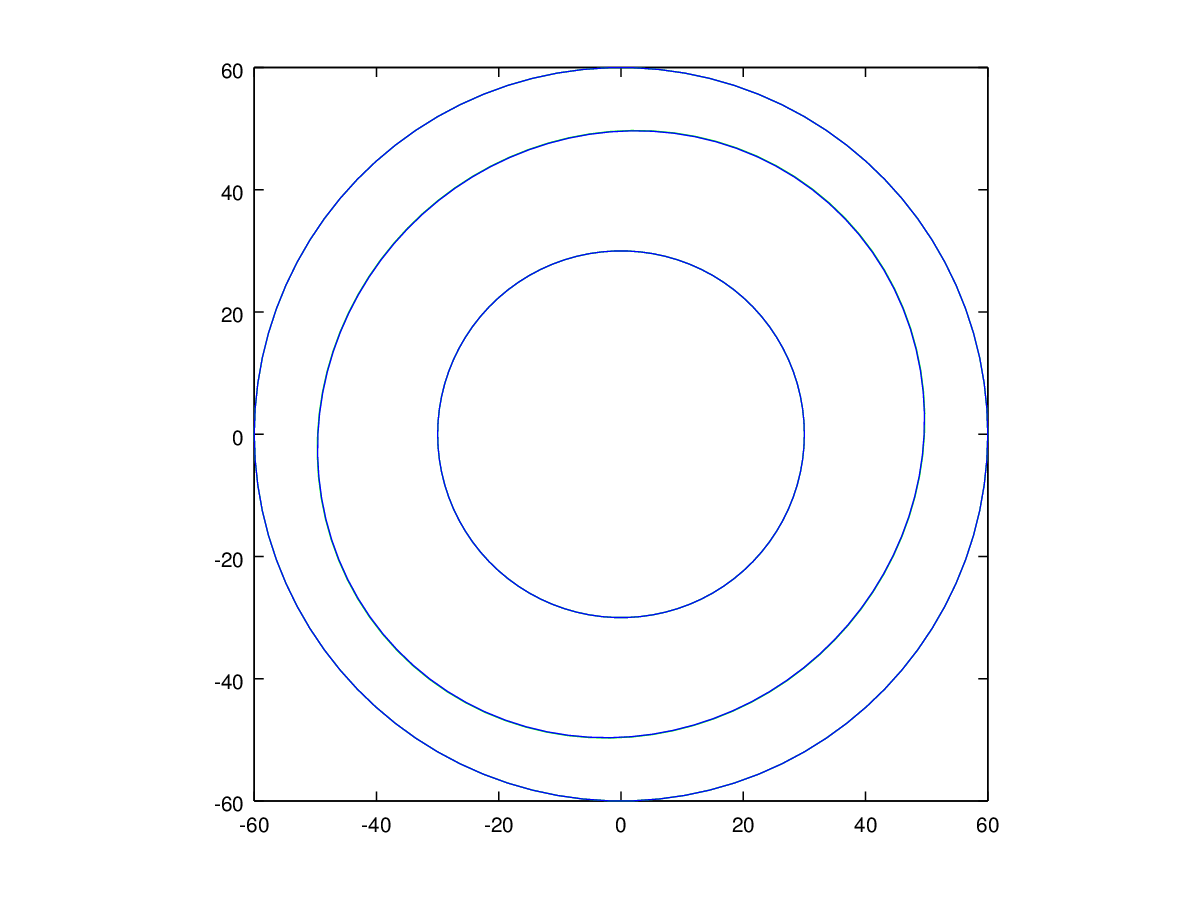
\includegraphics[width=4.5cm]{graficos/1/1b-8-iso.png} &
      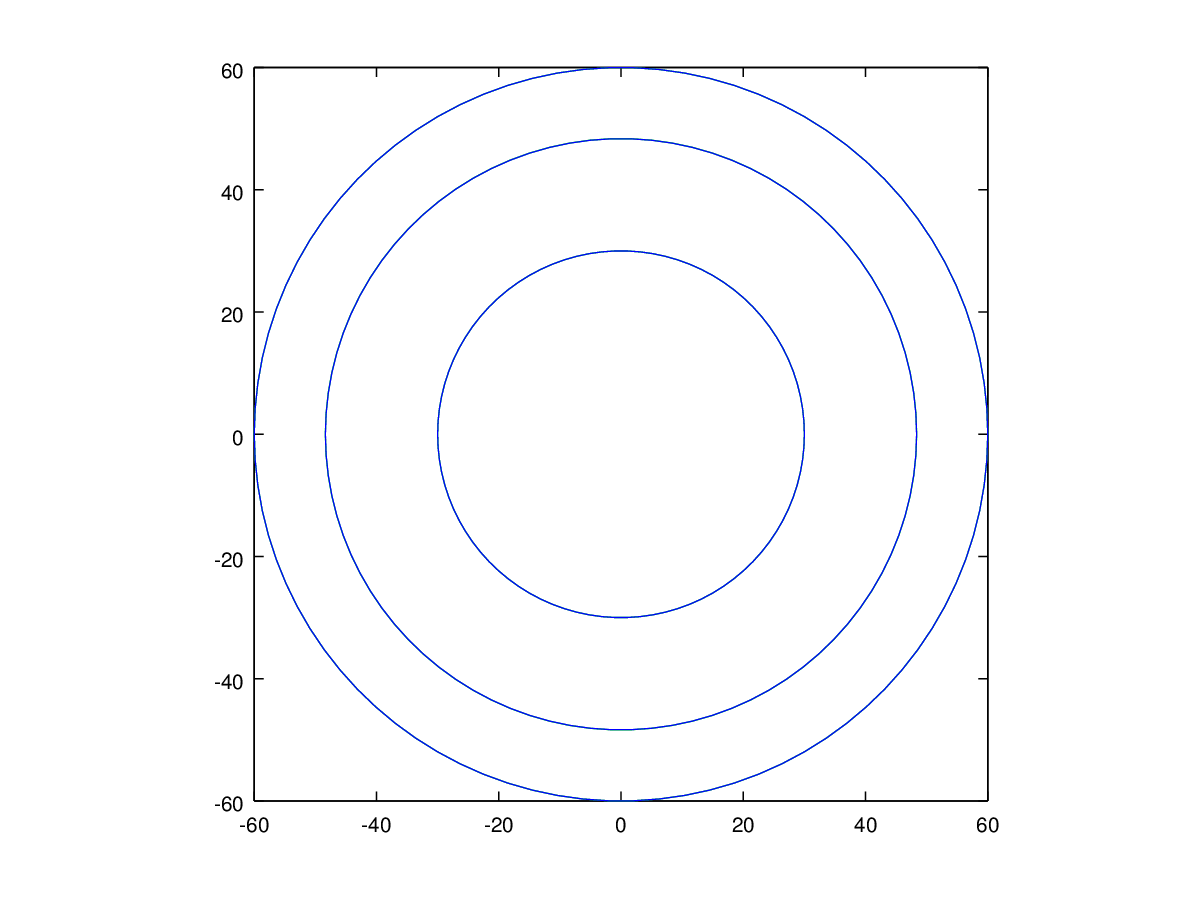
\includegraphics[width=4.5cm]{graficos/1/1b-30-iso.png} \\
      {\small $n = 3$} &
      {\small $n = 8$} &
      {\small $n = 30$} \\
    \end{tabular}}

  \subsubsection*{Experimento 3: Posición de la isoterma según condiciones de borde}

    

  \subsubsection*{Experimento 4: Índice de peligrosidad según granularidad}

  \subsubsection*{Experimento 5: Índice de peligrosidad según ancho de la pared}

  \subsubsection*{Experimento 6: Tiempo de ejecución según número de instancias}

  \subsubsection*{Experimento 7: Tiempo de ejecución según granularidad}


	
	
	


	\subsubsection*{Experimento 4}
	Se observa que cuando hay pocas instancias, buscar la isoterma con el metodo de eliminacion gaussiana o el de factriazacion LU es muy similar. A medida que aumentan las instancias las diferencias entre ambos metodos aumentan, ya que la factorizacion LU se mantiene casi inmutable al aumentar las instancias mientras que la eliminacion gaussiana aumenta notoriamente. Se puede observar que lo que tarda la eliminacion gaussiana cuando tiene 2 instancias es aproximadamentre el doble de lo que tarda cuando es una unica instancia. Cuando son 3 instancias, tarda el triple de lo que tarda cuando es una unica instancia. Entonces saean n instancias entonces lo que tarda la elimimacion gaussiana es lo que tarda cuando es una unica instancia * n. Esto es asi ya que en este metodo numerico, para cada una de las instancias recalcula toda la matriz. En cambio la factorizacion LU, calcula la matriz una unica vez.
  	
	\subsubsection*{Experimento 3}
	


  {\color{Gray} Deben incluir los resultados de los experimentos, utilizando el formato más adecuado para su presentación. Deberán especificar claramente a qué experiencia corresponde cada resultado. No se incluirán aquí corridas de máquina.}
